%\documentclass[11pt,a4paper,twoside]{tesis}
% SI NO PENSAS IMPRIMIRLO EN FORMATO LIBRO PODES USAR
\documentclass[12pt,a4paper]{tesis}

\usepackage{graphicx}
\usepackage[utf8]{inputenc}
\usepackage{pdflscape}
\usepackage[spanish]{babel}
\usepackage[left=3cm,right=3cm,bottom=3.5cm,top=3.5cm]{geometry}

\begin{document}

%%%% CARATULA

\def\autor{Christian Sebastian Russo}
\def\tituloTesis{Analysis of neighborhoods where it is convenient to build houses or buildings.}
\def\runtitulo{La Guerra de las Galaxias: Rebelión e Imperio}
\def\runtitle{Star Wars: Rebellion and Empire}
\def\director{Coursera Capstone}
\def\codirector{IBM Data Science Capstone}
\def\lugar{Buenos Aires, 2020}
\newcommand{\HRule}{\rule{\linewidth}{0.2mm}}
%
\thispagestyle{empty}

\begin{center}\leavevmode

\vspace{-2cm}






\vspace{6.0cm}

%\vspace{3.0cm}
%{
%\Large \color{red}
%\begin{tabular}{|p{2cm}cp{2cm}|}
%\hline
%& Pre-Final Version: \today &\\
%\hline
%\end{tabular}
%}
%\vspace{2.5cm}

\begin{huge}
\textbf{\tituloTesis}
\end{huge}

\vspace{2cm}


\vspace{2cm}

{\Large \autor}

\end{center}

\vfill

{\large

%{ \director}

\vspace{.2cm}

%{ \codirector}

\vspace{.2cm}

\lugar
}

\newpage\thispagestyle{empty}


%%%% ABSTRACTS, AGRADECIMIENTOS Y DEDICATORIA

\cleardoublepage
\tableofcontents

\mainmatter
\pagestyle{headings}

%%%% ACA VA EL CONTENIDO DE LA TESIS

\chapter{Introduction}
In Argentina, many construction companies have problems finding the best neighborhood to build houses or buildings.\\
This is because the places to build have different prices, but not only that, but it also depends on the commercial movement of the neighborhood, companies, industries, proximity to transport, shops, businesses, among others.\\\ \\
On the other hand, the construction of a house is not the same as that of a building, the commercial and movement analysis of an area is different.\\ \\
It is for this reason that different companies have difficulty and ask themselves: What is the best place to start a new venture? \\ \\

\chapter{Description of the problem}
In the \textbf{Buenos Aires} province there are neighborhoods where a property costs around USD 70,000, in turn near this property we can find a property with similar characteristics at USD 200,000, that is, a price of \textbf{285 \%} highest.\\ \\
The price of a property is given, among other things, by the proximity to places of interest; for example, a property near a supermarket / shopping that is close to a cemetery will not have the same price. \\ \\
Among many of the factors that are taken into account when choosing \textit{where} the venture is considered more feasible, is the proximity to different points of interest, such as: shops, supermarkets, bars, train stations, bus stations, avenues, etc.


\chapter{Solution approach}
In the present work, the first thing we will do is obtain the necessary geographic information of the neighborhoods of \textbf{Buenos Aires} (correctly called departments) to be able to work with the API of \textit{Foursquare} in order to obtain the points of interest of each neighborhood. \\
Once this information is obtained, we will calculate, for each neighborhood, what proportion of each category of places of interest counts, finally calculating a total value (the sum of the percentages of each category) and thus be able to measure how feasible it is to build in that neighborhood. \\

Then, we will use the algorithm of \textbf{Machine Learning} (called \textit{k-means}) to be able to determine similarities between neighborhoods, and with these similarities find a neighborhood similar to another with the desired characteristics.

The desired points of interest that we will use in these examples are:

\begin{itemize}
\item Train stations
\item Shops
\item Restaurants
\item Gyms
\item Places
\item Airports
\item Cinemas
\item Shoppings
\item Supermarkets
\item Bars
\item Clubs
\item Etc.
\end{itemize}




Finally, we will analyze a particular neighborhood, evaluating in which areas within it, the commercial movement is greatest.

\chapter{Data analysis}
The first thing we will do is analyze the data obtained from \textit{https://www.datos.gob.ar/}. Once the data in Buenos Aires and Capital Federal has been filtered, the result of those data from the neighborhoods of Argentina will be shown. \\
\\
\\
\centerline{
	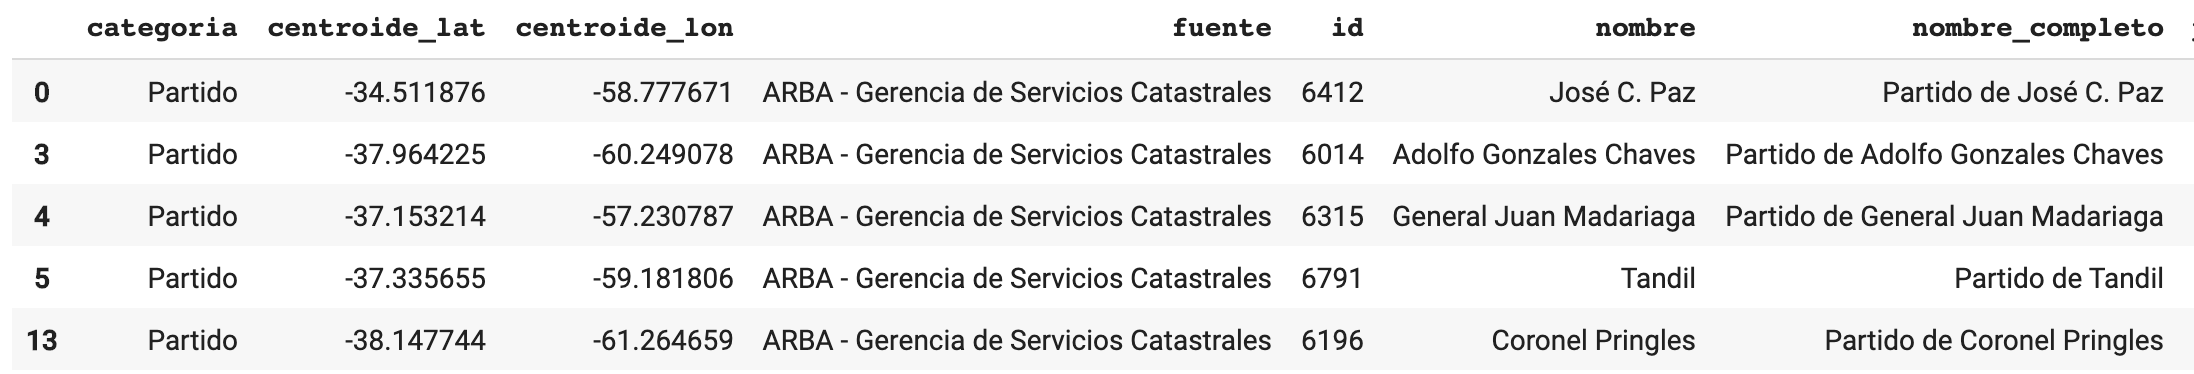
\includegraphics[scale=0.36]{tabla1}
}
\\
\\

Using the geographic coordinates of each neighborhood (latitude and longitude) we will draw a map to verify the information obtained: \\ \\

\centerline{
	\includegraphics[scale=0.3]{mapa1}
}

\begin{landscape}

\centerline{
	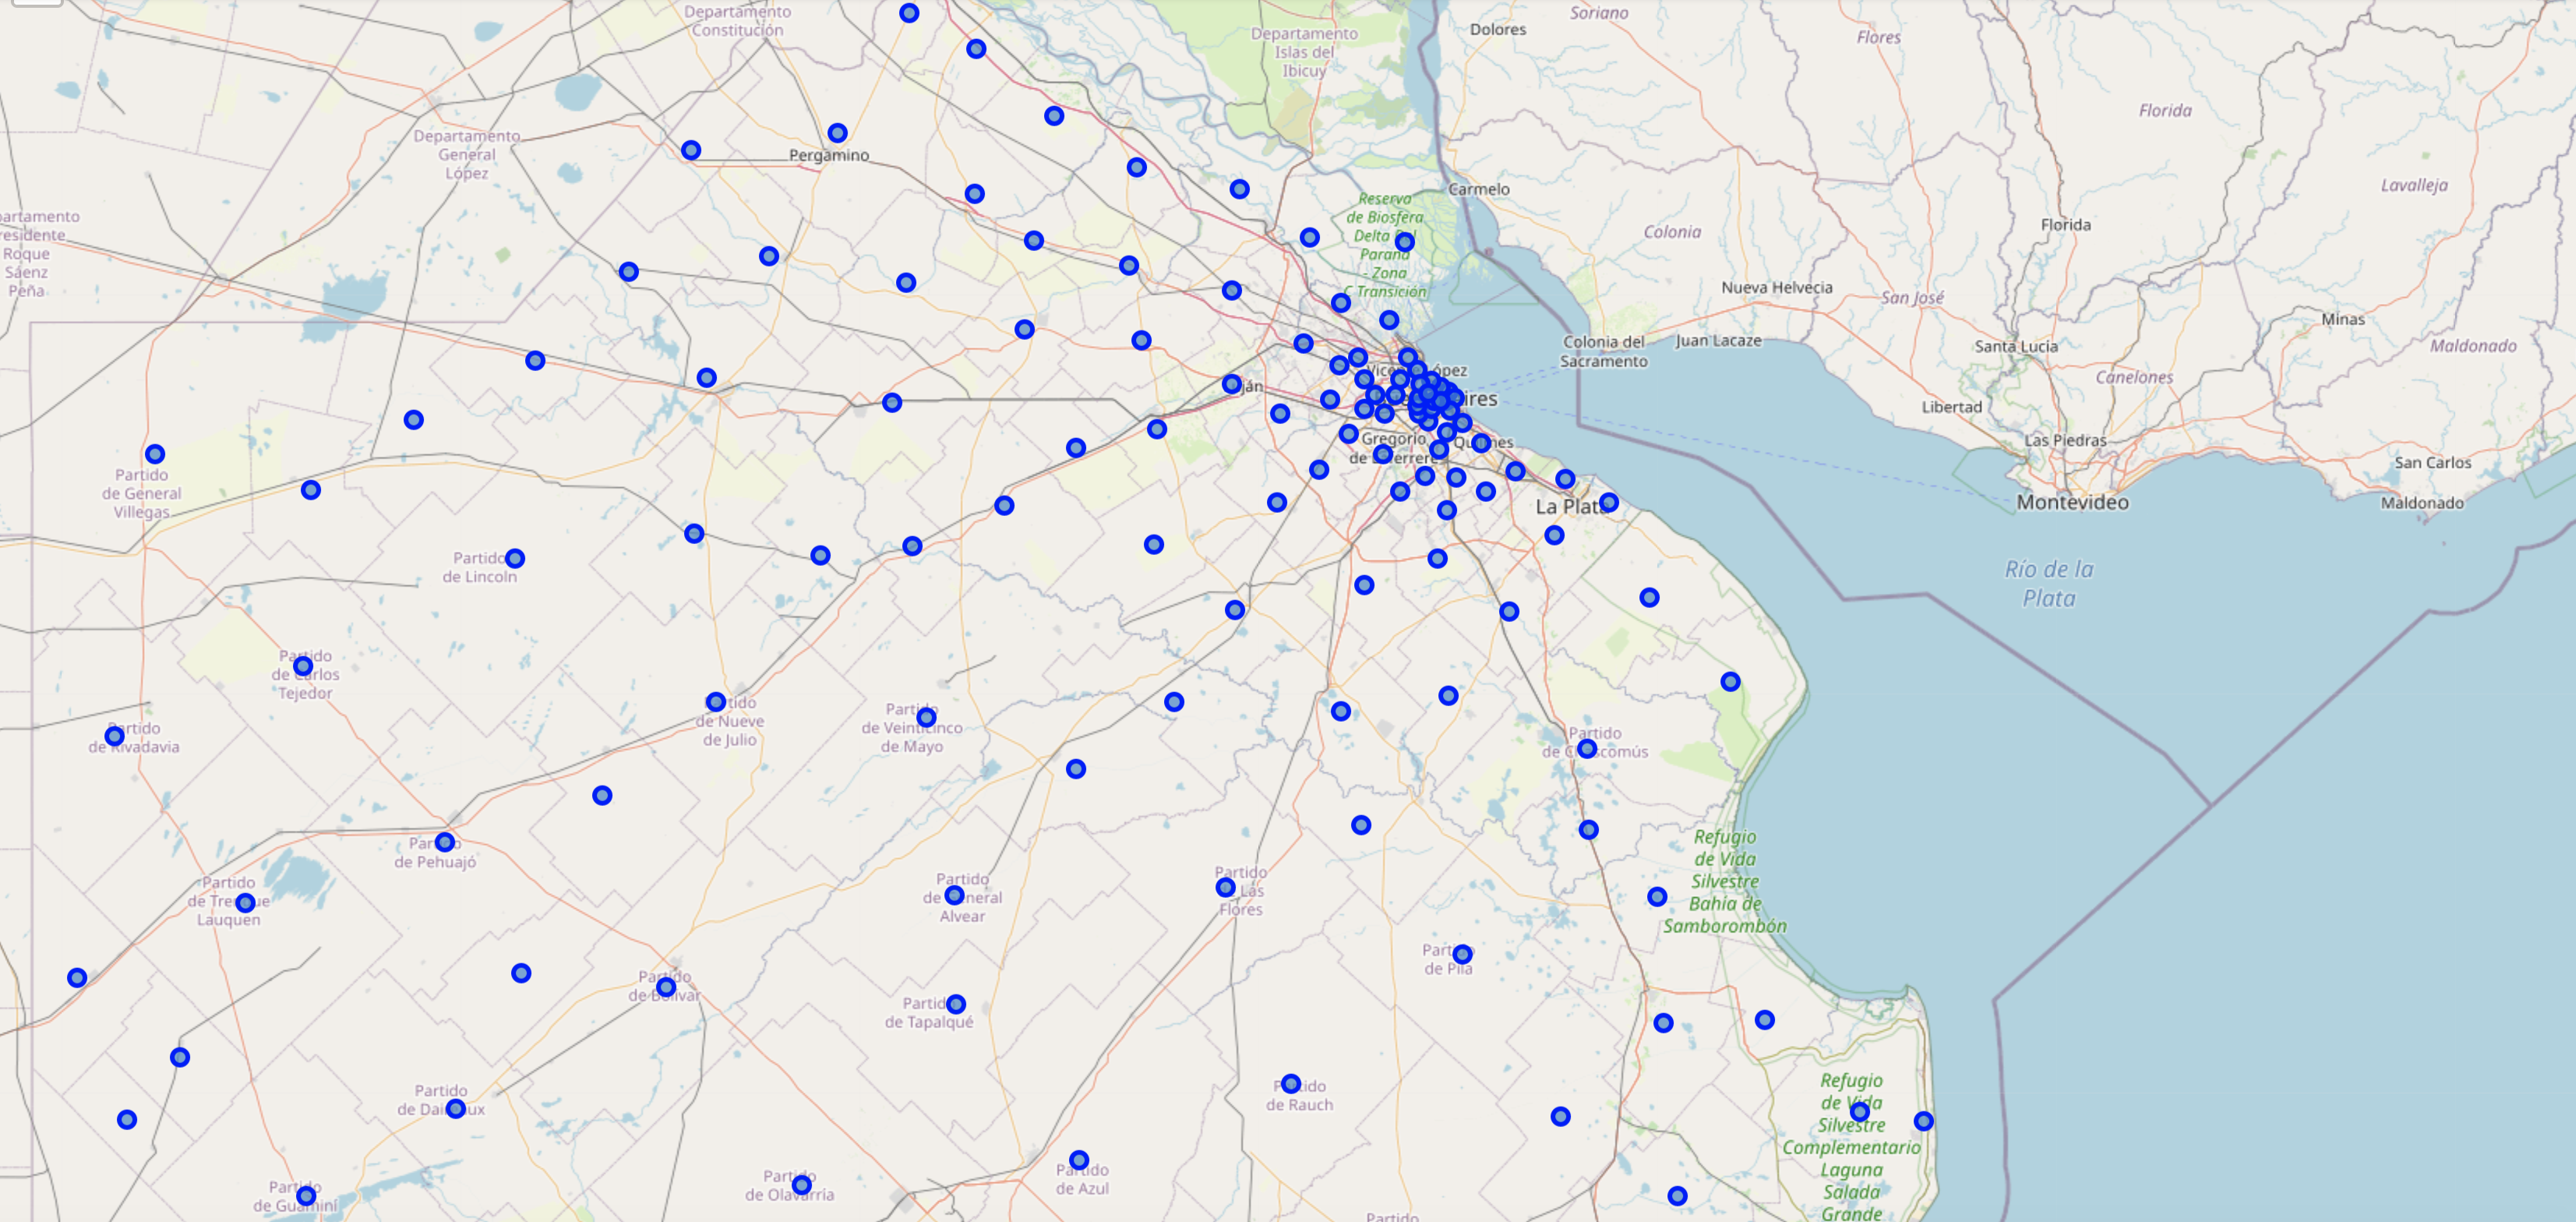
\includegraphics[scale=0.25]{mapa2}
}

\centerline{
	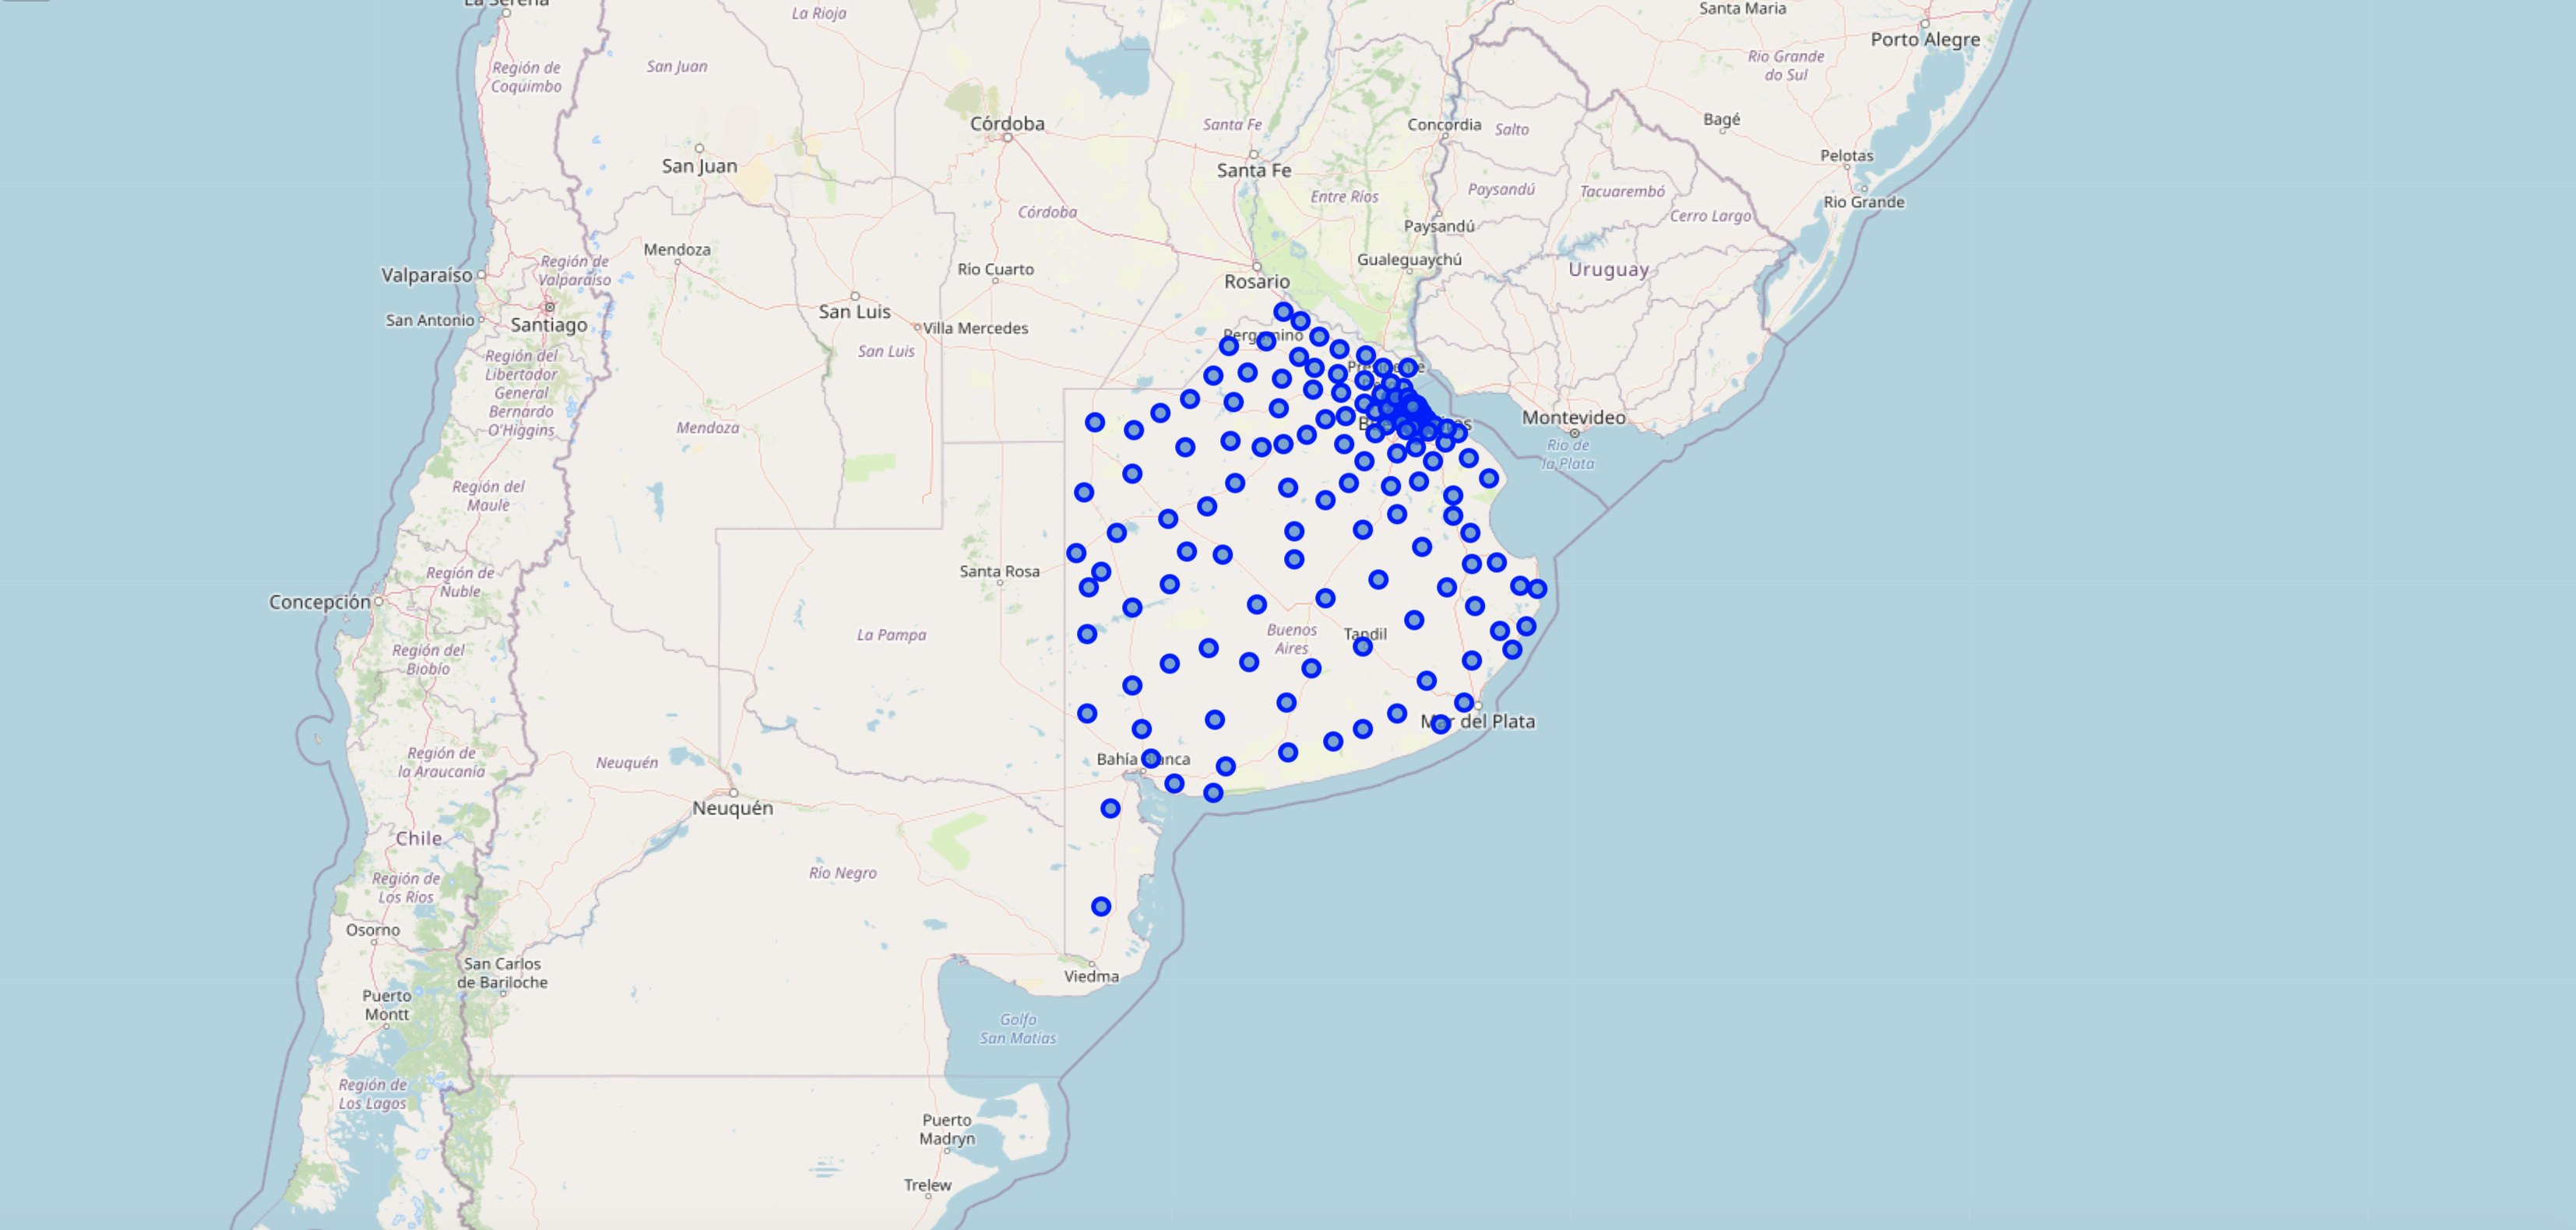
\includegraphics[scale=0.25]{mapa3}

}
\end{landscape}

As you can see on the three maps, all the neighborhoods in the province of Buenos Aires are represented with blue circles.
\\ \\
Then, using the Foursquare API (https://api.foursquare.com/v2/venues/explore), we will calculate for each neighborhood its points of interest. \\
Note, that for the use of the API we need to configure a limit and radius of results for each neighborhood. For this instance we will configure the radius at 8000 meters and the limit of results at 500 units. \\
Once the API was used, we found 3904 points of interest, and for each of these its category, latitude, longitude, name, type, etc. \\
Finally, what we will do, using the One Hot Encoding technique and grouping data will be to generate a table that for each neighborhood we can see how many points of interest it has separated by category. \\

Let's see a part of the table: \\ \\

\centerline{
	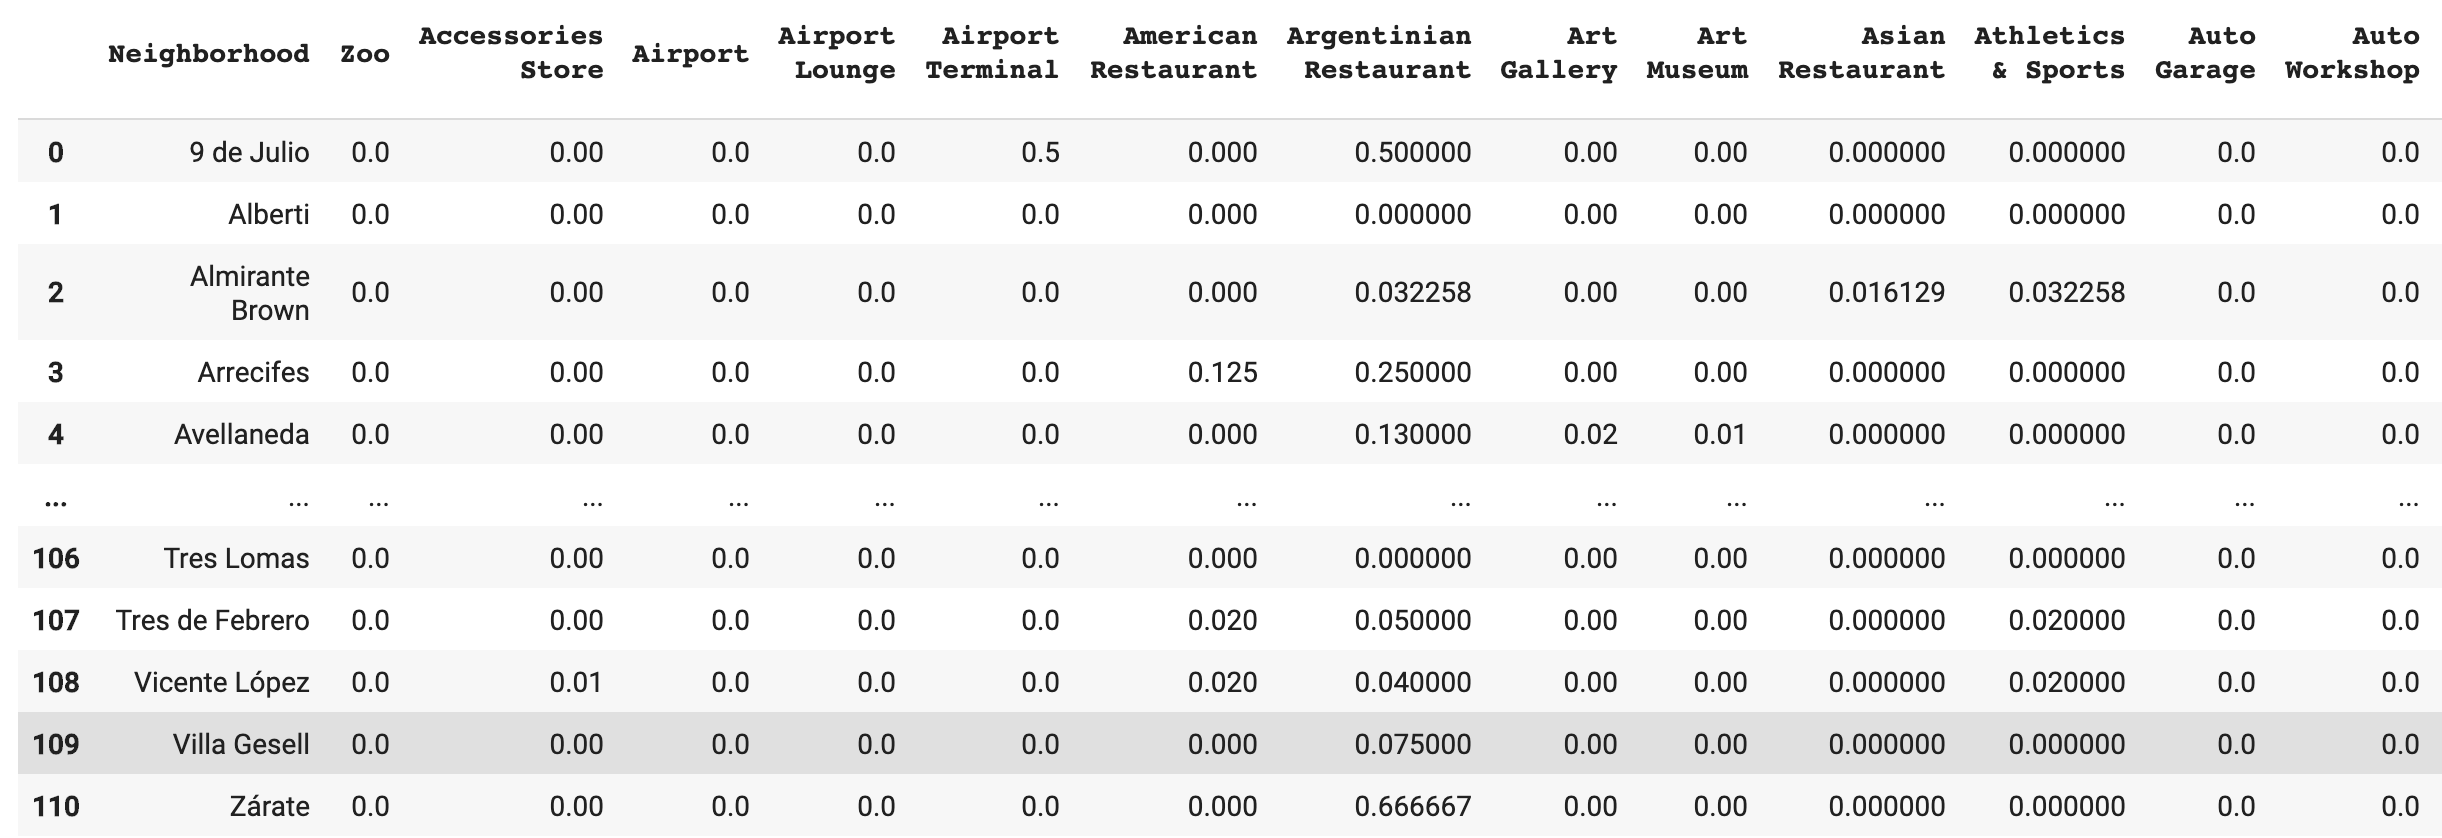
\includegraphics[scale=0.4]{tabla2}
}
As you can see in the table, we have an average value in each category grouped by neighborhood. \\
For example, we can see that for July 9, 0.5 of the results obtained are Argentine Restaurants. \\
\\
After this, we will add the information in the table for all the neighborhoods, to obtain a value per neighborhood and be able to draw it obtaining the following graph. It is important to note that not all the categories were added, but only the desired category:

\centerline{
	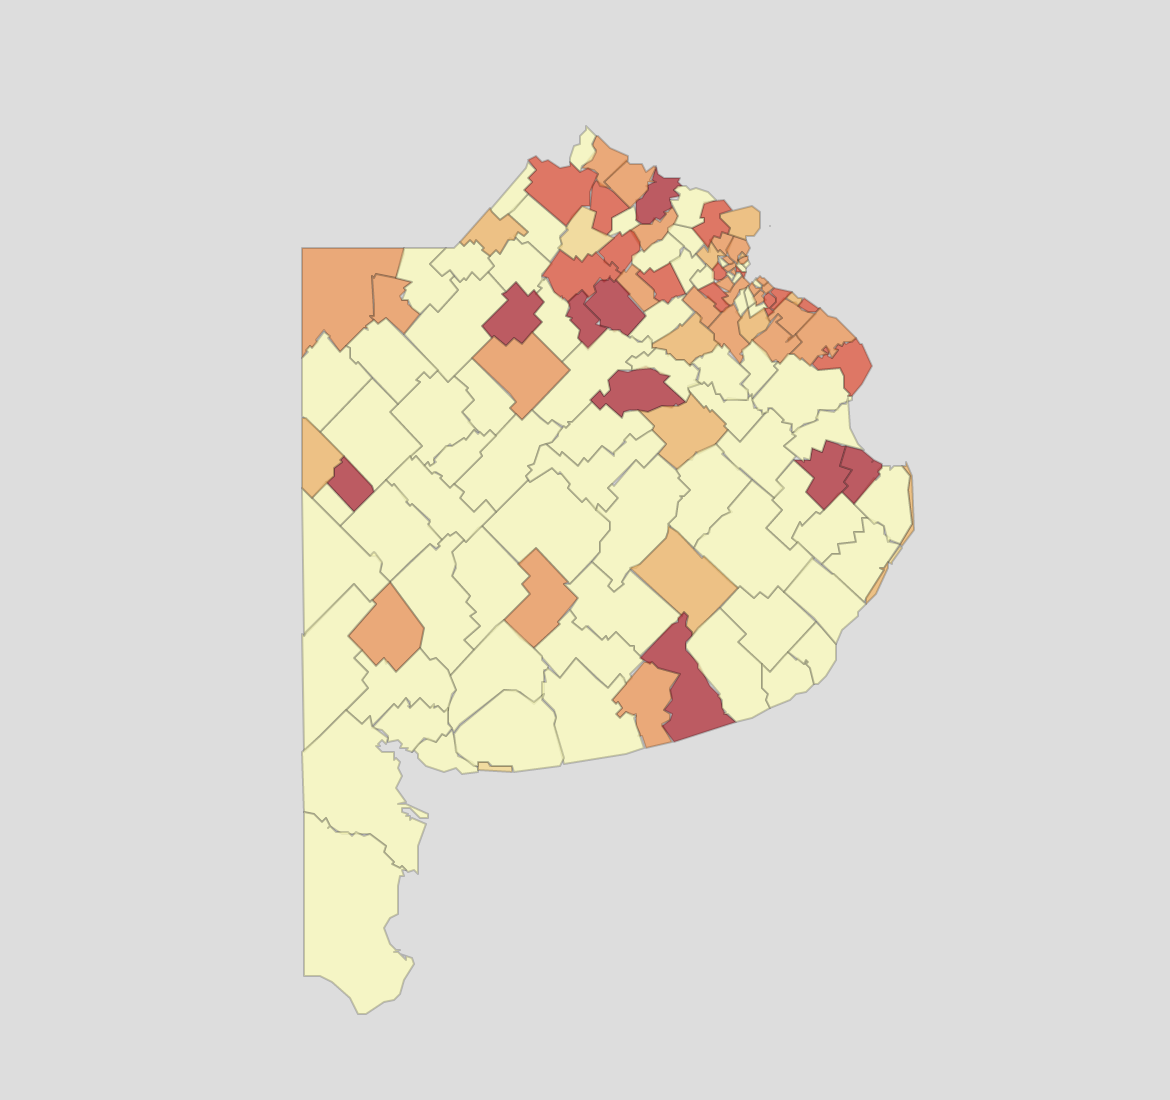
\includegraphics[scale=0.8]{mapa4}
}

Also on the map you will see the neighborhoods where the desired categories are more frequent in red and therefore we consider it a neighborhood with more movement according to our wishes. \\

It is interesting to note that with this information we could, given a neighborhood, know which categories of points of interest are more frequent, for example let's see the results in the Hurlingham neighborhood:

\begin{center}
 \begin{tabular}{||c c ||} 
 \hline
 Point of interest & Value \\ [0.5ex] 
 \hline\hline
 Ice Cream Shop & 0.13 \\ 
 \hline
 Argentinian Restaurant & 0.12 \\
 \hline
 Cafe & 0.07  \\
 \hline
 Plaza & 0.04  \\
 \hline
 Bar & 0.03  \\ [1ex] 
 \hline
\end{tabular}
\end{center}


\chapter{Cluster Neighborhood}
With the Machine Learning algorithm called KMeans, we will generate 5 clusters to be able to find similarity between different neighborhoods, this could help construction companies in their analysis and thus determine where it is convenient for them to invest. \\
We will add to the tables the results of our algorithm so as to have, given a neighborhood id, to which cluster it belongs, as we see in the following table: \\ \\
\centerline{
	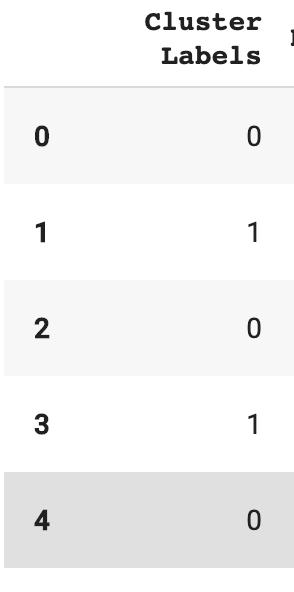
\includegraphics[scale=0.5]{tabla3}
}

To better see the results and see the clusters of our algorithm, we draw it on the map: \\ \\

\centerline{
	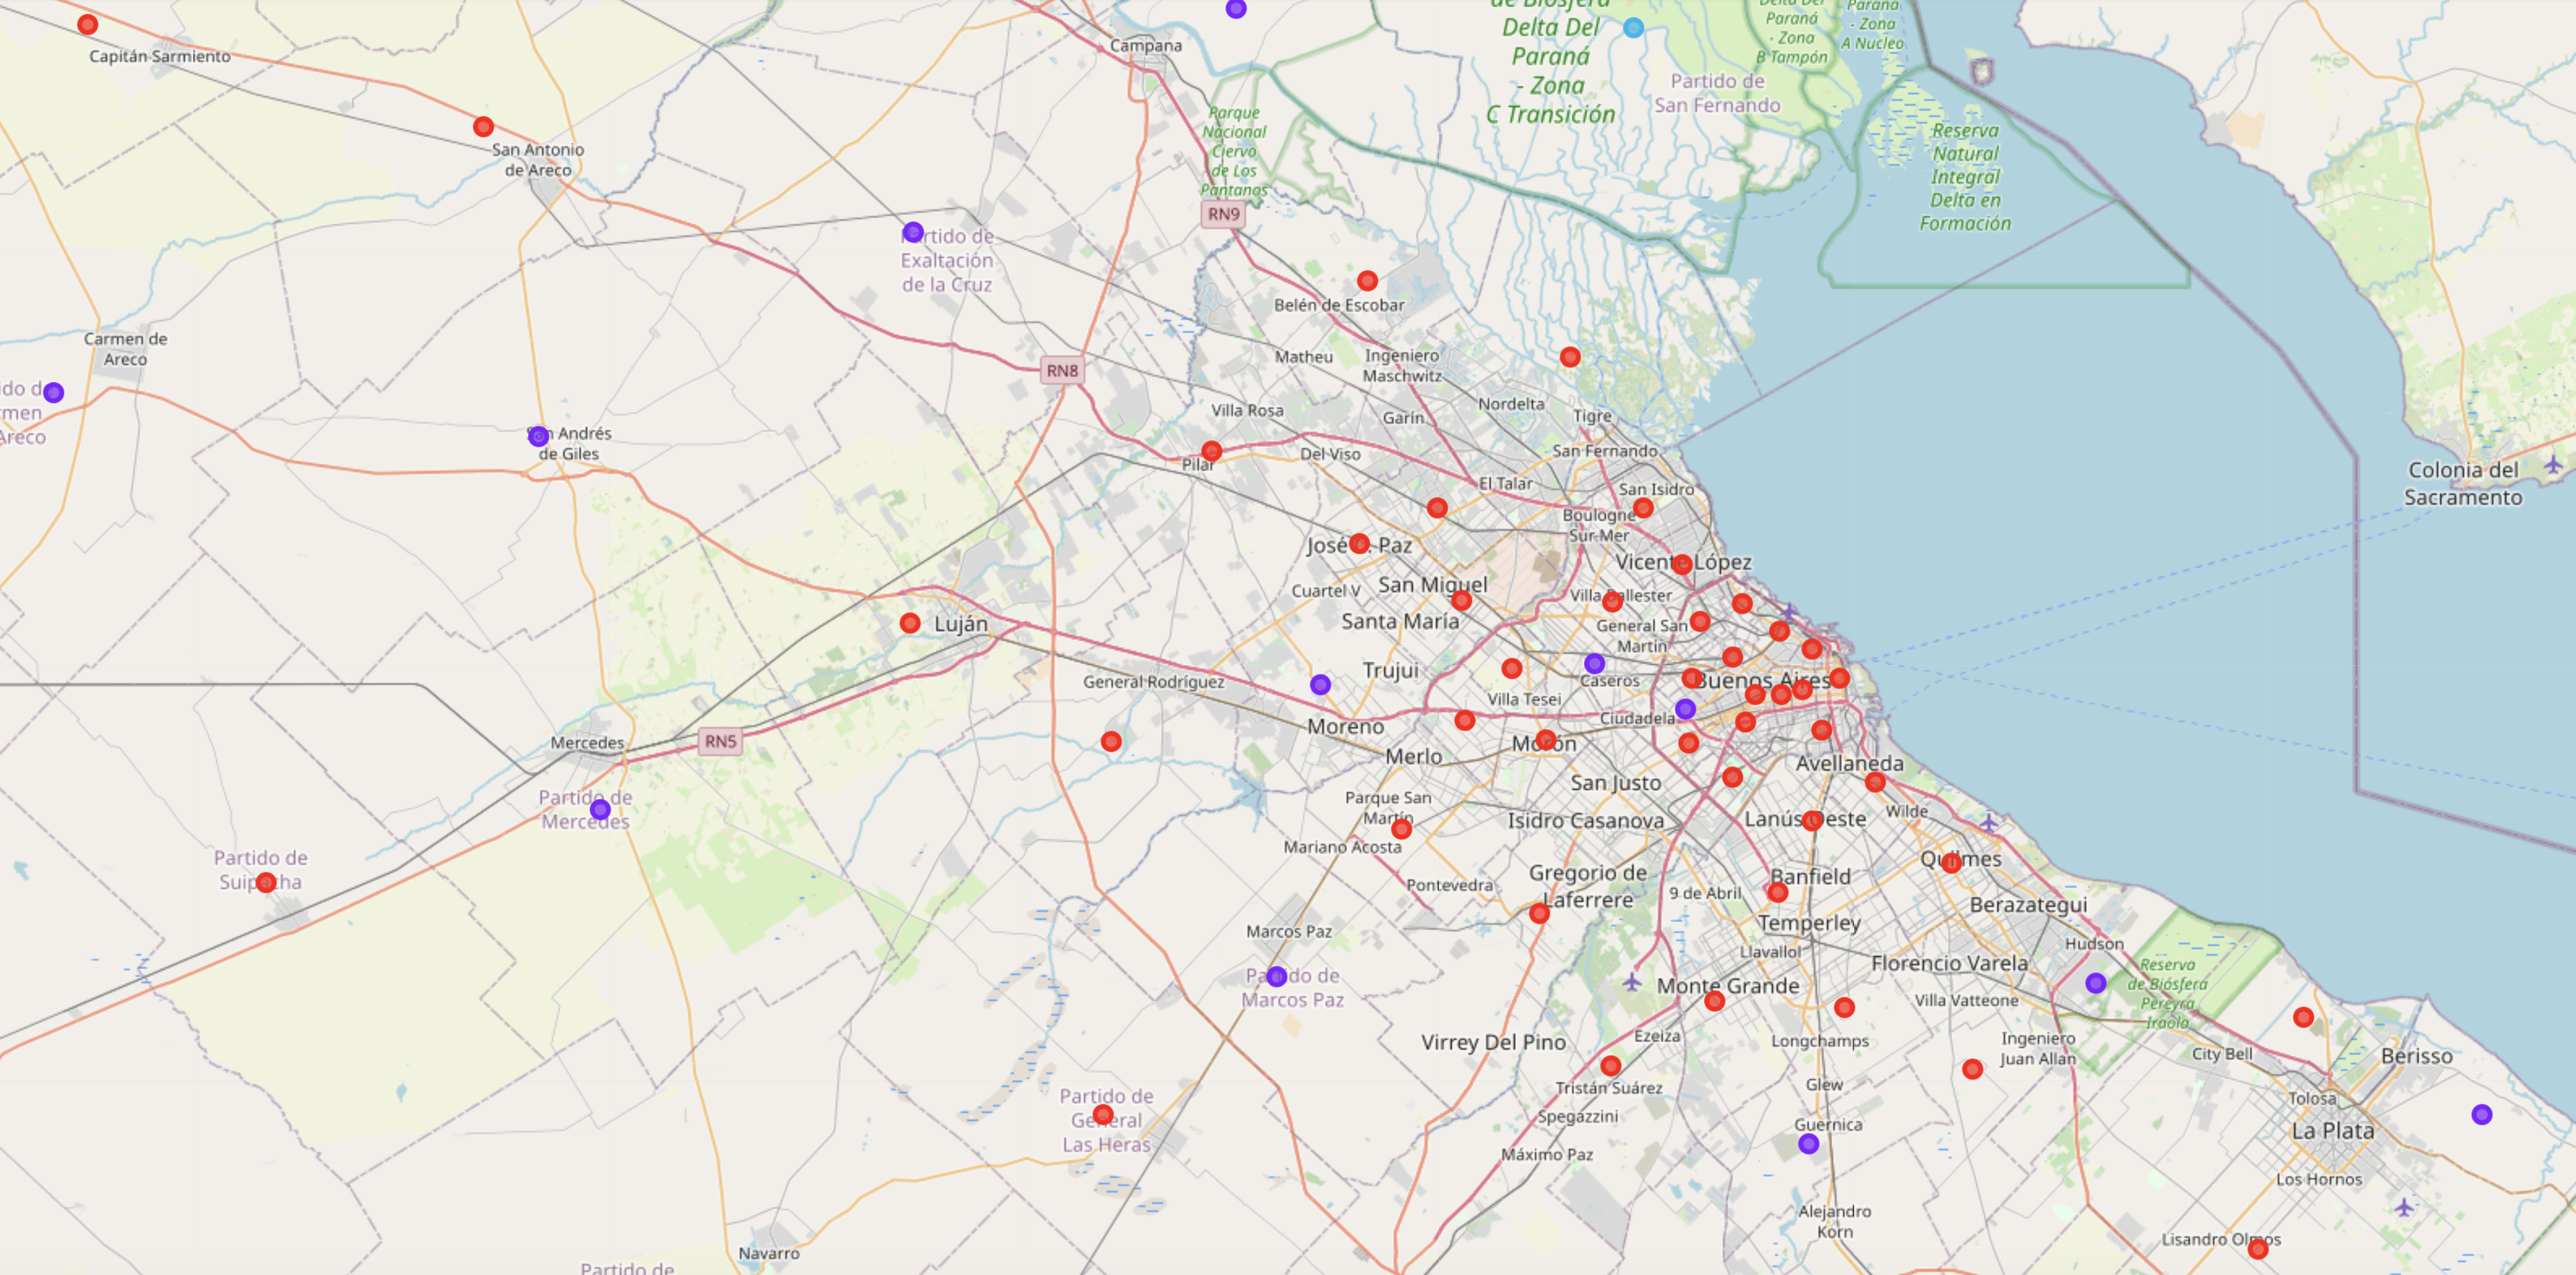
\includegraphics[scale=0.3]{mapa5}
}

\centerline{
	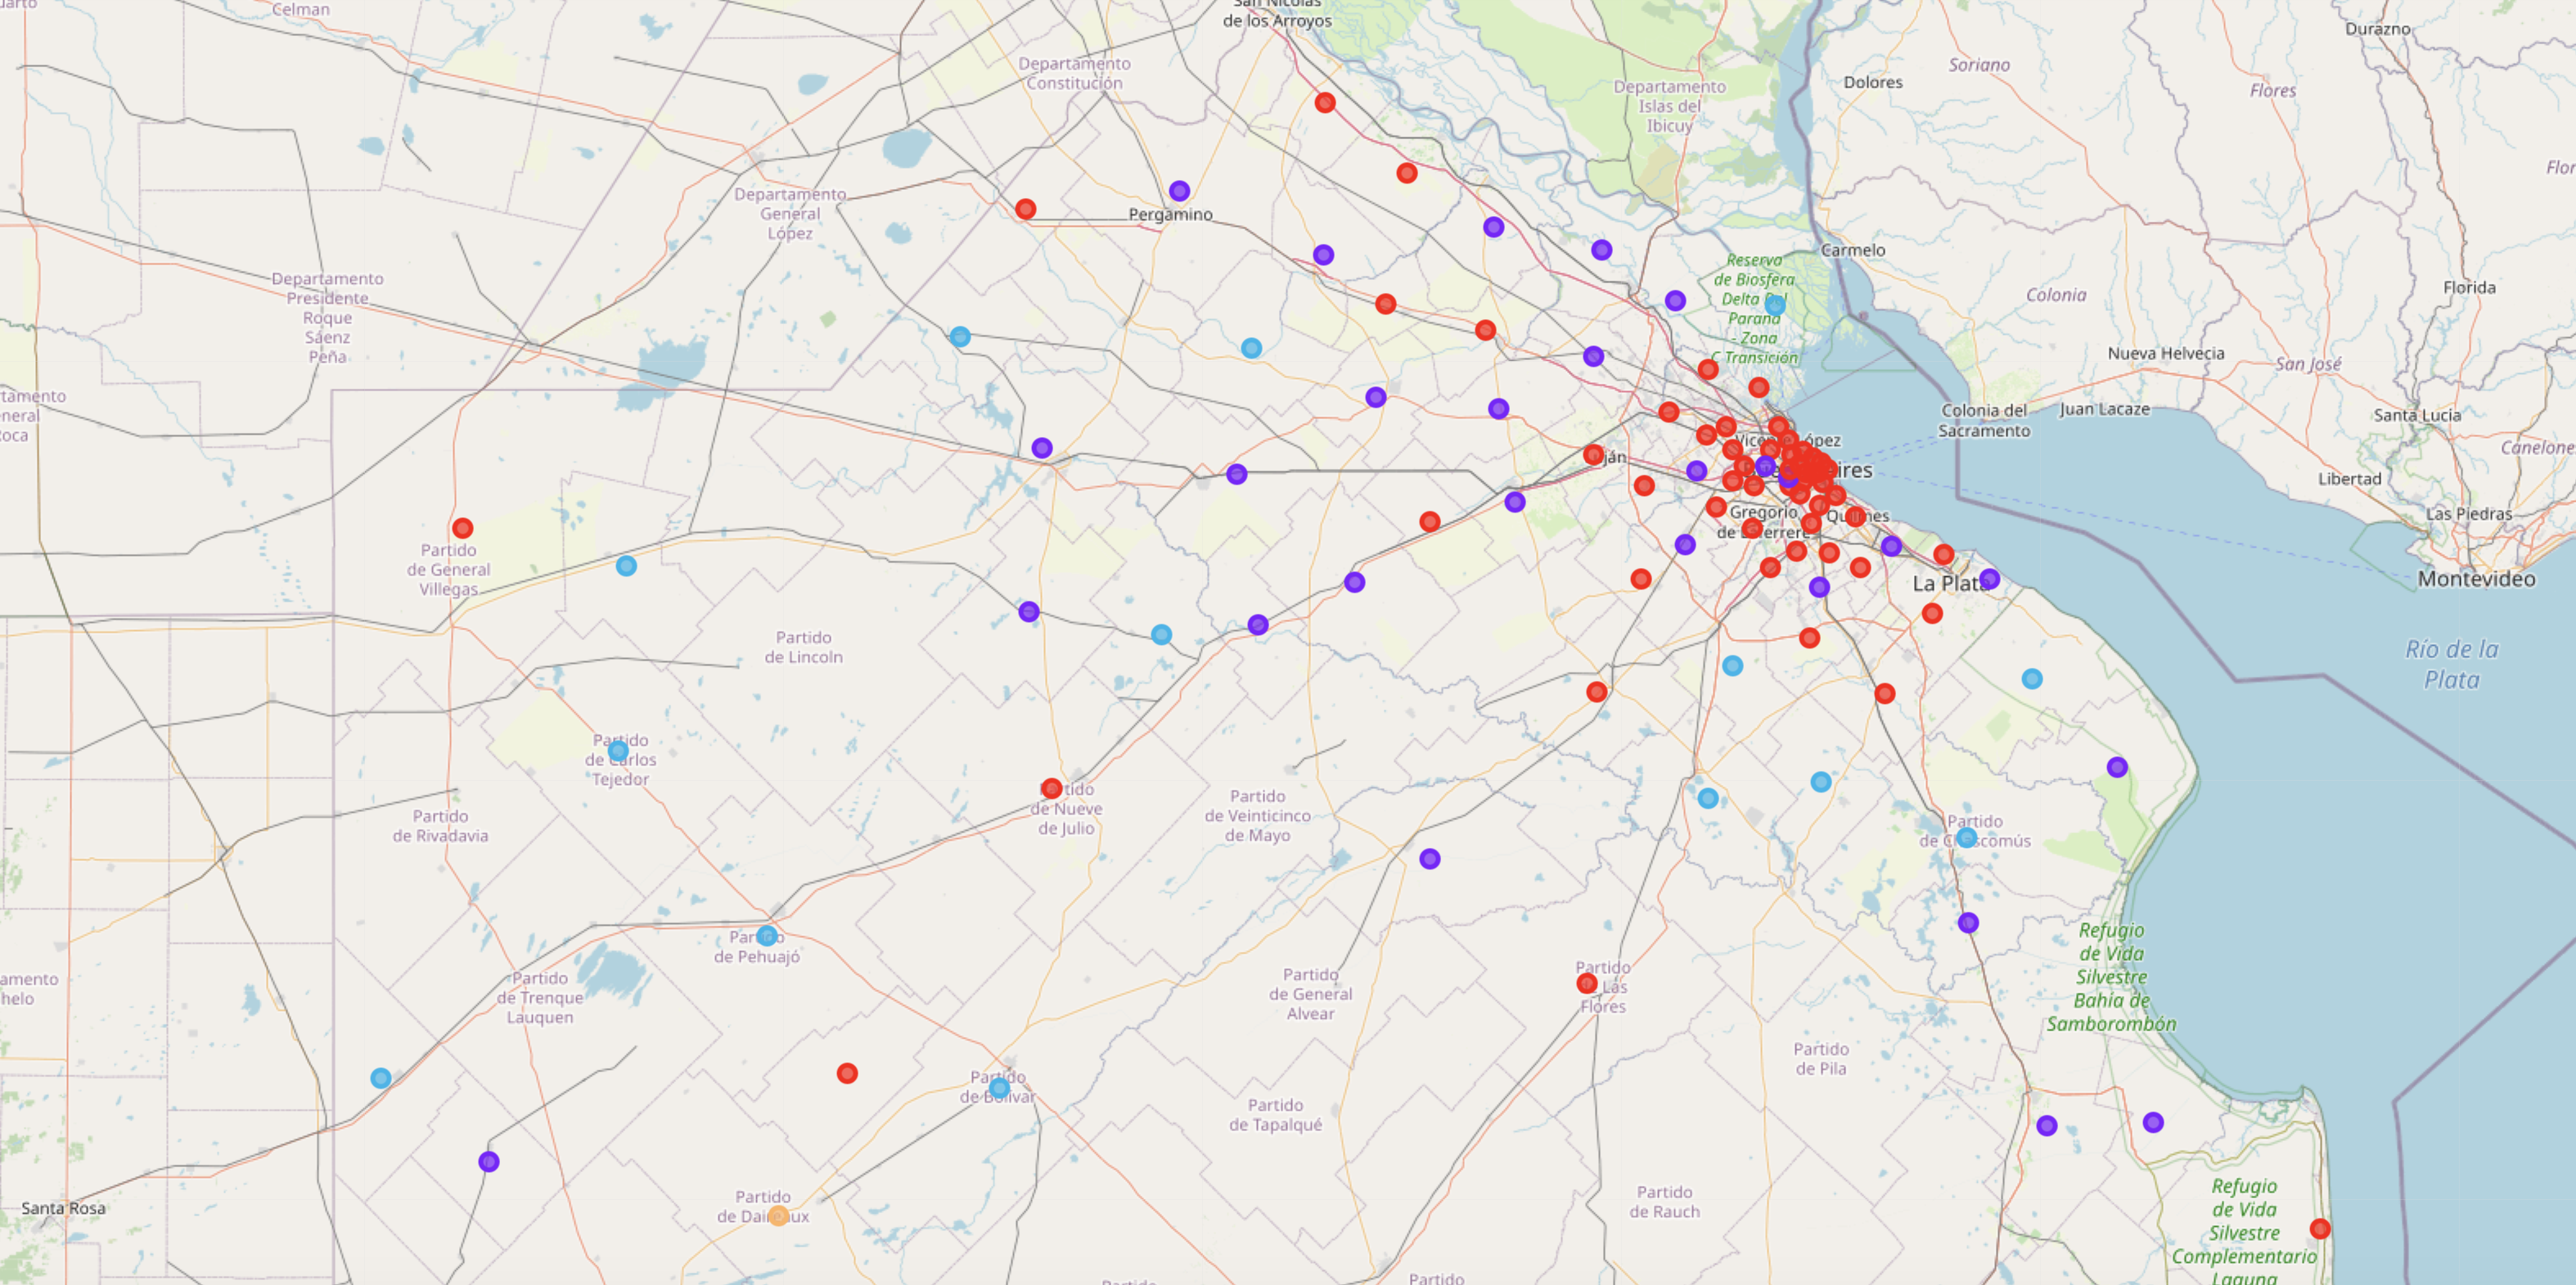
\includegraphics[scale=0.3]{mapa6}
}

\centerline{
	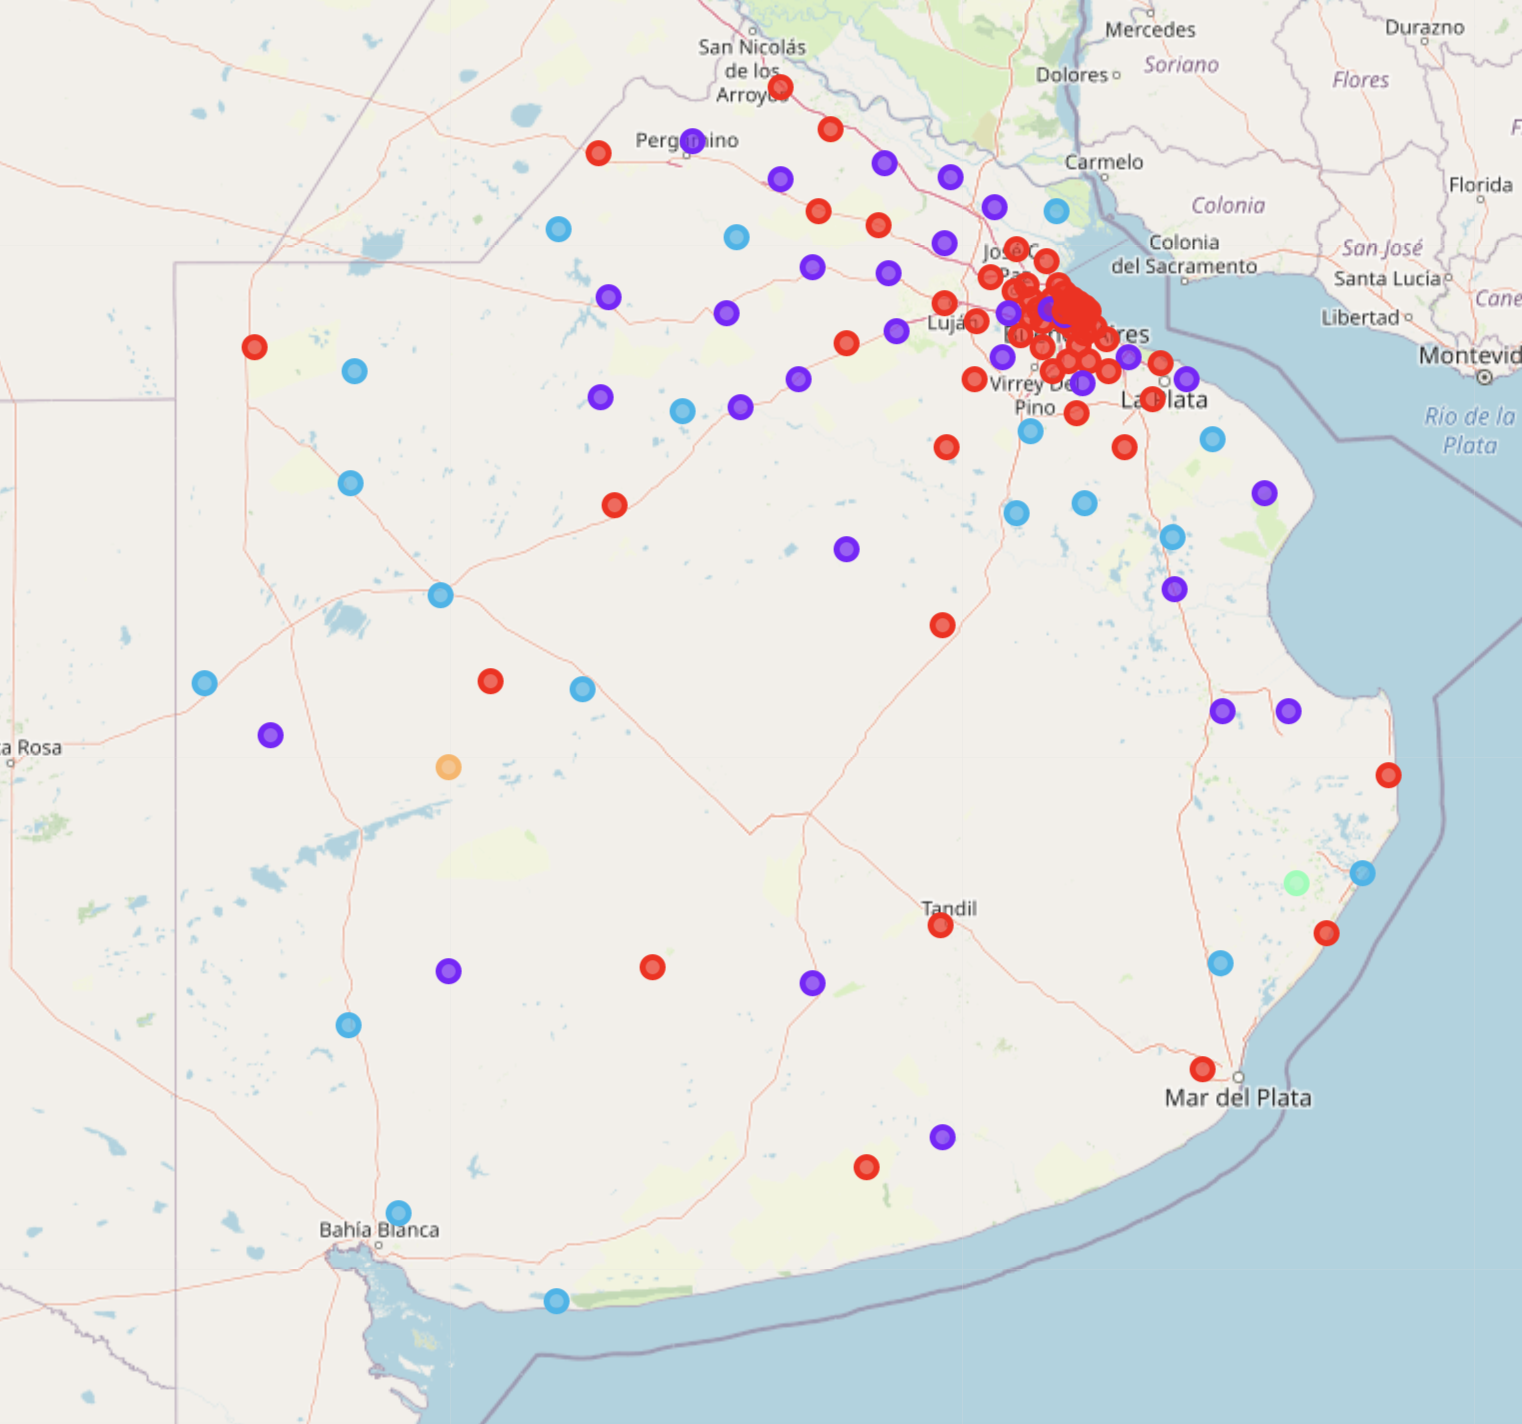
\includegraphics[scale=0.3]{mapa7}
}

In the maps, we observe that all the points of the same color are the neighborhoods that we consider to be similar in the movement of the points of interest selected. \\

Now, let's analyze the same algorithm but with 10 clusters and see the results obtained:

\centerline{
	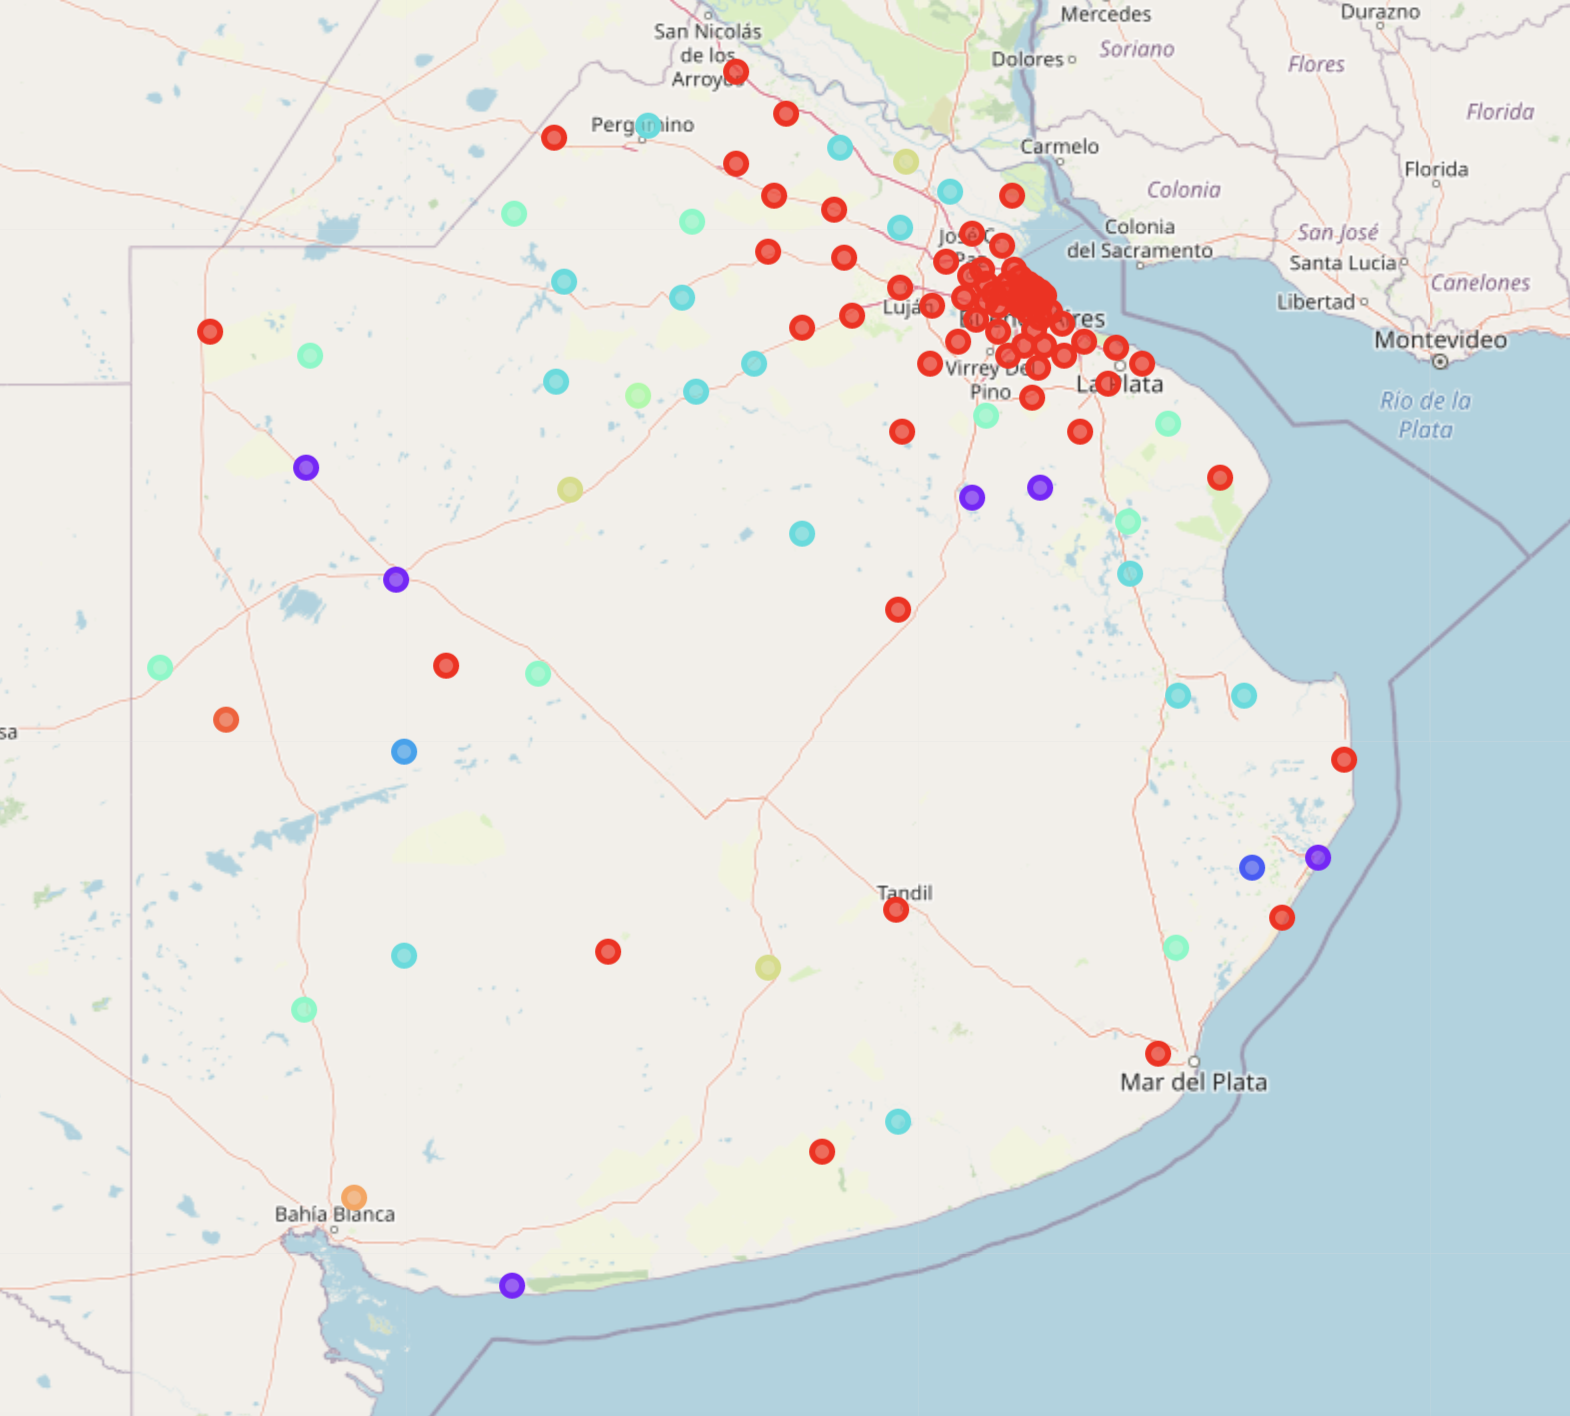
\includegraphics[scale=0.5]{mapa8}
}

\newpage
Finally, let's evaluate with a number of clusters equal to 100. \\ \\


\centerline{
	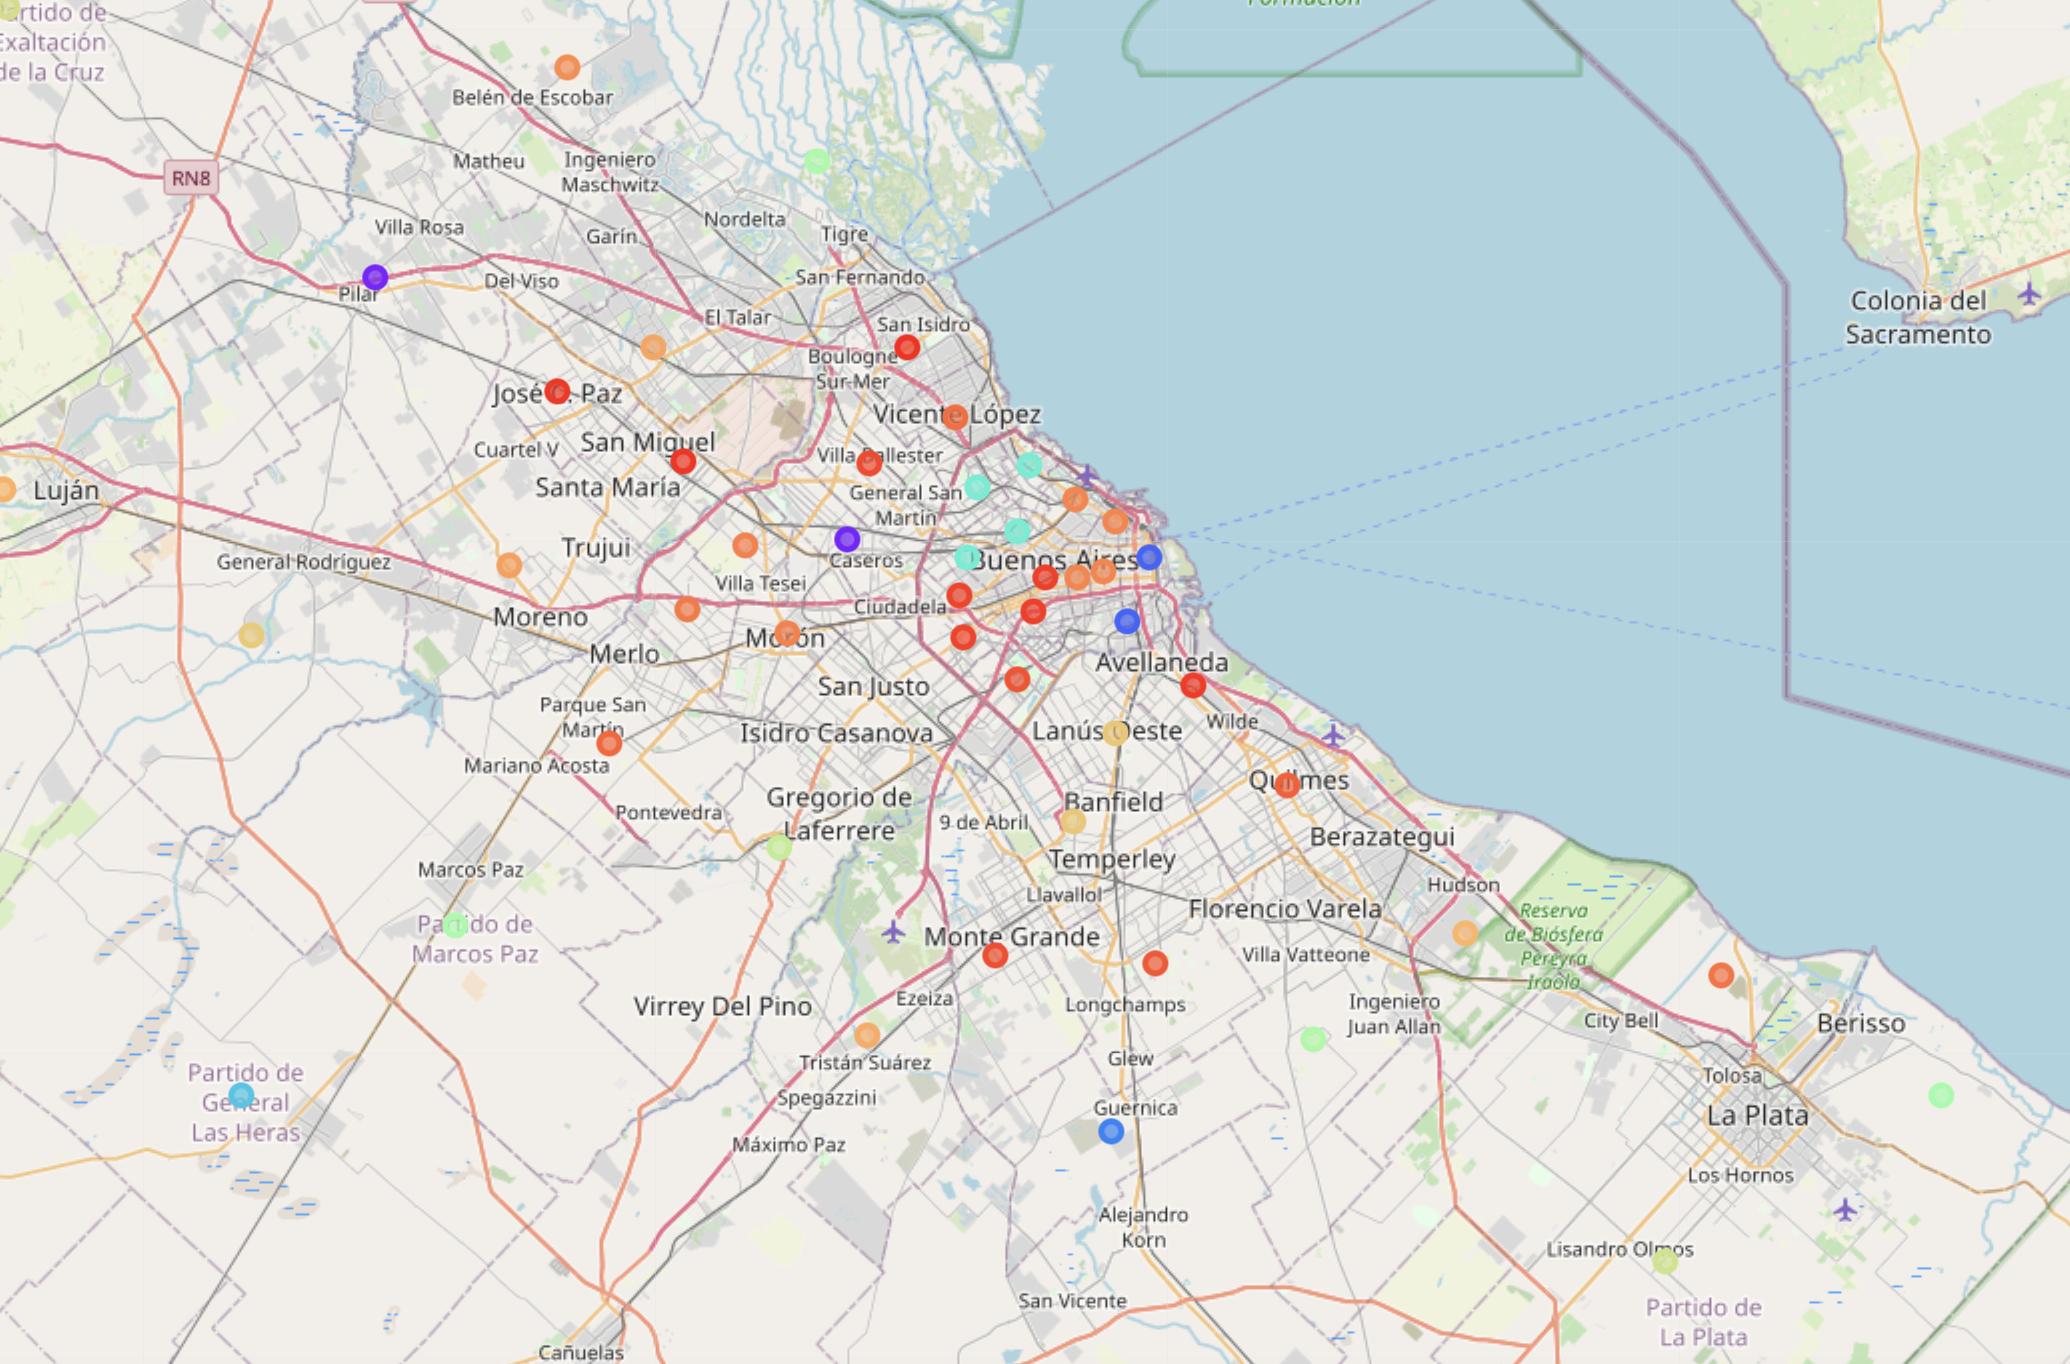
\includegraphics[scale=0.45]{mapa9}
}


\centerline{
	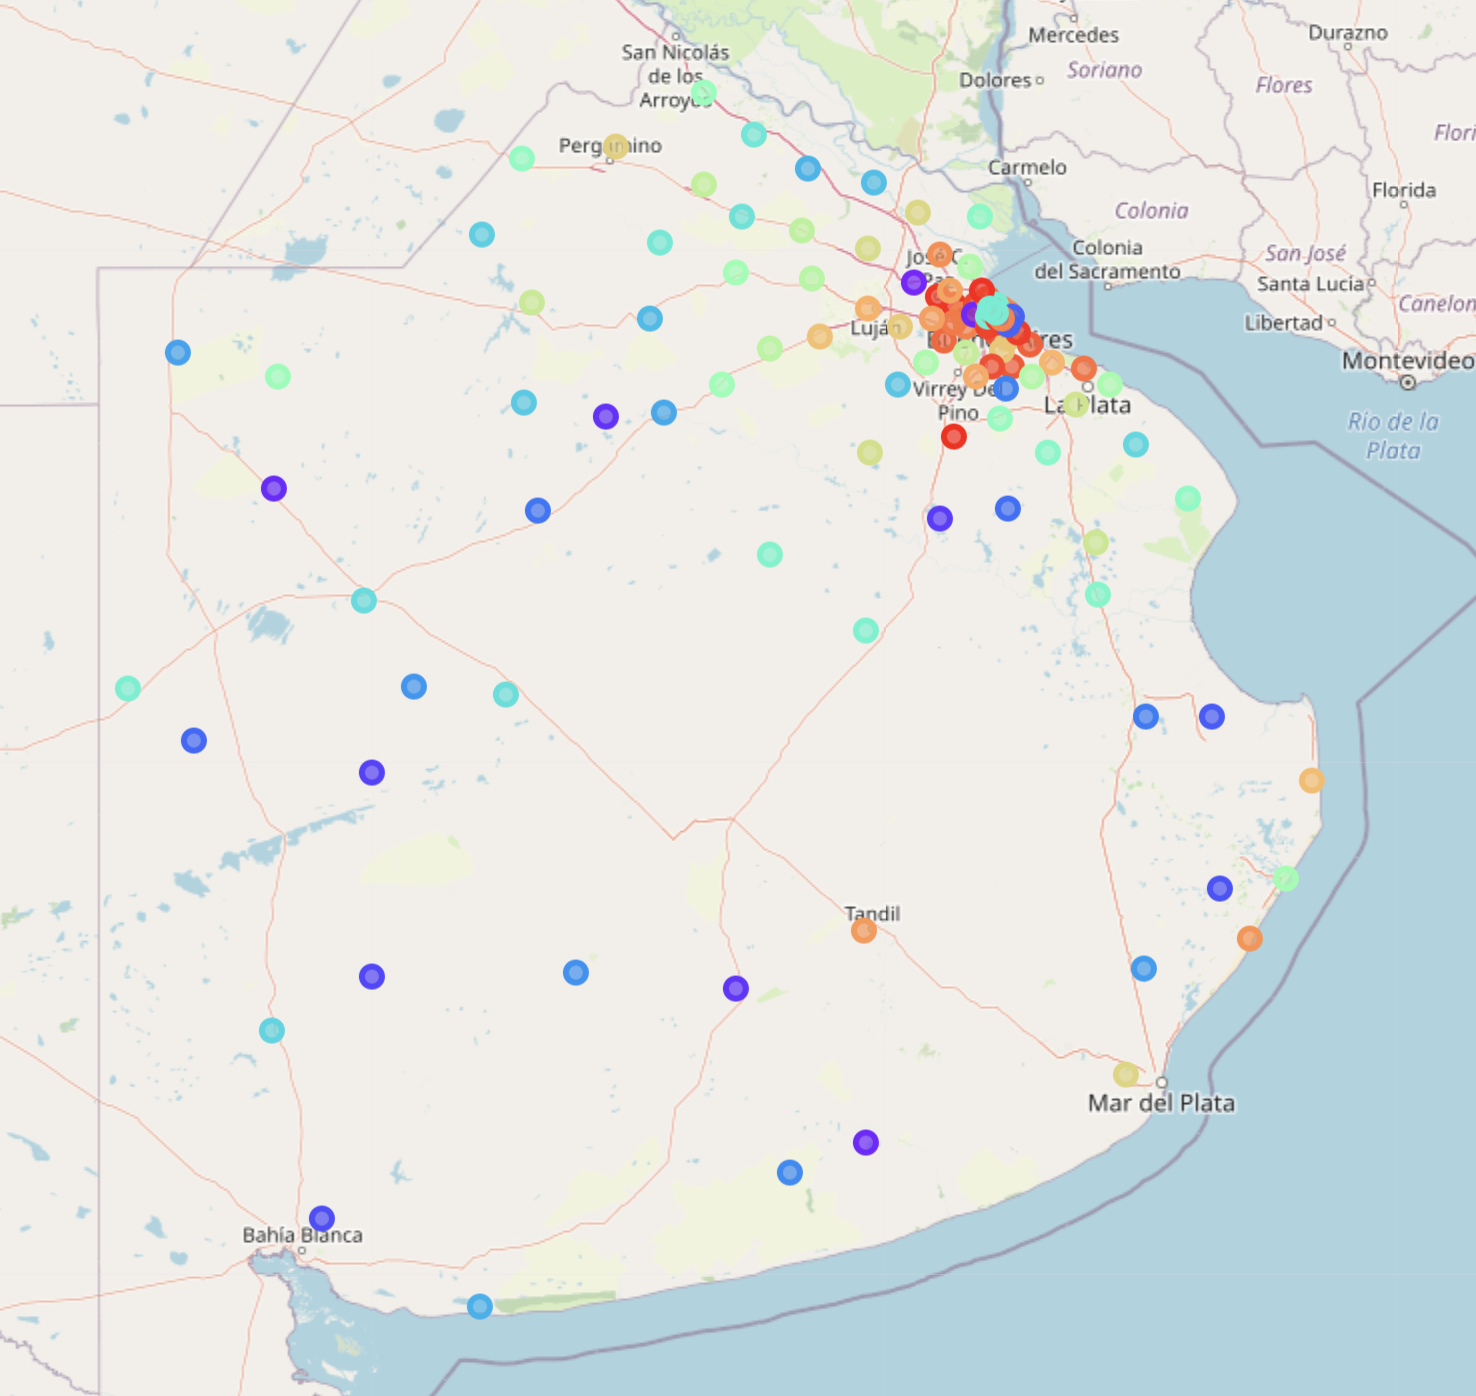
\includegraphics[scale=0.4]{mapa10}
}

\chapter{Analysis of a particular neighborhood}
In this chapter we will evaluate the same logic used in the previous chapter, but instead of the entire province of Buenos Aires, we will only take the neighborhood called \textbf{Morón}. \\

The first thing we will do is determine the geographical limits of the neighborhood and obtain its polygon. \\ \\

\centerline{
	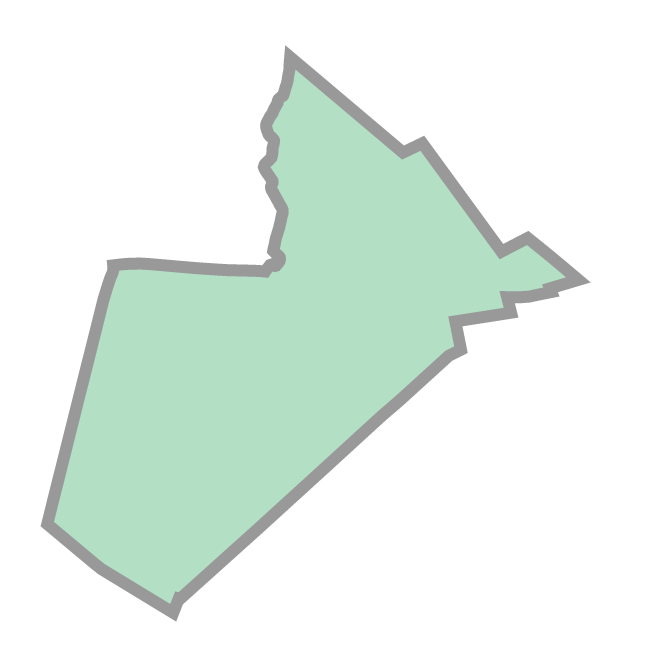
\includegraphics[scale=0.5]{moron}
}

Then we will generate random points within the limits of the neighborhood. For this example we will execute only 20 points.

We repeat the previous process, that is, we generate a table with One Hot Encoder and group by a unique identifier (in this case we use the tuple made up of latitude and longitude as the identifier). We calculate the total sum of the percentages of movement at each point of interest and make it on a map.

\centerline{
	\includegraphics[scale=0.3]{mapa11}
}

On the map, you can see the marked points and the radius is equivalent to the percentage of movement of the point. That is, the more radius the circle has centered on the point, it is because that point has more movement than the desired points of interest. \\ \\

Now let's try 40 new random points: \\

\centerline{
	\includegraphics[scale=0.35]{mapa12}
}

\chapter{Conclusion}
In this work we could see that the Foursquare API is very powerful and it gives us very detailed information on all the areas that we will want. It was also possible to observe a great difficulty when analyzing the data, since when mixing data from different sources they are not always perfectly equal. \\
An interesting conclusion is that the way to calculate the movement of a point of interest can not only be given by the sum of its percentages (this is a way that we evaluate in this report only), it is left for future work to investigate better ways of calculating this value. \\
Looking at maps of Buenos Aires we can see that the places with the most movement are coincidentally the most populated and closest to the capital, or for general knowledge, places that are heavily traveled. \\
It is very interesting to know for a neighborhood, how populated it is with certain categories of points of interest, we believe that this data is useful in different studies. \\
Using Machine Learning we saw that the places closest to the capital and with the most movements are very similar to each other, while places in the interior are not. We also believe that as the number of clusters increased, this similarity changed for the better. \\

Analyzing data from the Moron neighborhood, we find the problem that being random points, they are not always the best, nor are they well located, therefore we believe that it would be a good starting point for a next job.


\chapter{Future works}
Outside of this report, the analysis of hyperparameters, that is, in Machine Learning algorithms, could evaluate the value of K (number of clusters) is more appropriate. \\

On the other hand, improve the use of the Foursquare API, since we remember that we use limits and radii that were configured very small to obtain the results more quickly. \\

Also, when calculating the mobility percentage of each neighborhood, a better heuristic or equation could be studied to obtain more general results. \\

Finally, an analysis of the price per square meter in each neighborhood could be added to the study. \\

\chapter{External links}
\begin{itemize}
\item https://www.datos.gob.ar/
\item https://es.foursquare.com/
\end{itemize}
\end{document}
